\documentclass[a4paper,twoside,11pt]{article}

%the preamble
\usepackage[]{geometry}
\geometry{
	total={155mm,257mm},
	left=20mm,
	top=20mm,
}

\usepackage{marginnote}


\usepackage{lipsum}                     % Dummytext
\usepackage{xargs}    
\usepackage{amsmath,amsfonts,mathabx}
\usepackage{epigraph}  


\usepackage{framed}
\usepackage{color}

\newenvironment{shadequote}%
{\begin{snugshade}\begin{quote}}
		{\hfill\end{quote}\end{snugshade}}


\definecolor{shadecolor}{rgb}{0.9,0.9,0.9}






%\epigraphfontsize{\small\itshape}
%\setlength\epigraphwidth{10cm}
\setlength\epigraphwidth{.8\textwidth}
\setlength\epigraphrule{0pt}


%#this make the epigraph box with italic text
\usepackage{etoolbox}
\makeatletter
\newlength\epitextskip
\pretocmd{\@epitext}{\em}{}{}
\apptocmd{\@epitext}{\em}{}{}
\patchcmd{\epigraph}{\@epitext{#1}\\}{\@epitext{#1}\\[\epitextskip]}{}{}
\makeatother







% Use more than one optional parameter in a new commands
\usepackage[pdftex,dvipsnames]{xcolor}  % Coloured text etc.
% 
\setlength{\marginparwidth}{2cm}
\usepackage[colorinlistoftodos,prependcaption,textsize=tiny]{todonotes}
\newcommandx{\unsure}[2][1=]{\todo[linecolor=red,backgroundcolor=red!25,bordercolor=red,#1]{#2}}
\newcommandx{\change}[2][1=]{\todo[linecolor=blue,backgroundcolor=blue!25,bordercolor=blue,#1]{#2}}
\newcommandx{\info}[2][1=]{\todo[linecolor=OliveGreen,backgroundcolor=OliveGreen!25,bordercolor=OliveGreen,#1]{#2}}
\newcommandx{\improvement}[2][1=]{\todo[linecolor=Plum,backgroundcolor=Plum!25,bordercolor=Plum,#1]{#2}}
\newcommandx{\thiswillnotshow}[2][1=]{\todo[disable,#1]{#2}}
%

\usepackage{blindtext} % for dummy text
% \usepackage[margin=2cm]{geometry}   % to change margins
% \usepackage{titling}             % Uncomment both to   
% \setlength{\droptitle}{-2cm}     % change title position 







%%%%%%%%%%%%%%%%%%%%%%%%%%%%%%%%%%%%%%%%%%%%%%%%%%%%%%%%%%%%%%%%%%%%%%%%%%%%%%%%%%%


%       Document to Start HERE


%%%%%%%%%%%%%%%%%%%%%%%%%%%%%%%%%%%%%%%%%%%%%%%%%%%%%%%%%%%%%%%%%%%%%%%%%%%%%%%%%%%





\author{Nam Le}
\title{%\vspace{-1.5cm}            % Another way to do
	Consulting Engineering: Constructing the future}

\begin{document}
\maketitle

\pagestyle{plain}

\section{Introduction}
Here goes a good animation

\marginnote{Well, if you dont have a good sense of humor, who you gonna become }[1cm]
\begin{figure}[!htb]
	\centering
	%	\includepdf[angle = 0]{sections/CHE_1PHSC_with_VFD.pdf}
	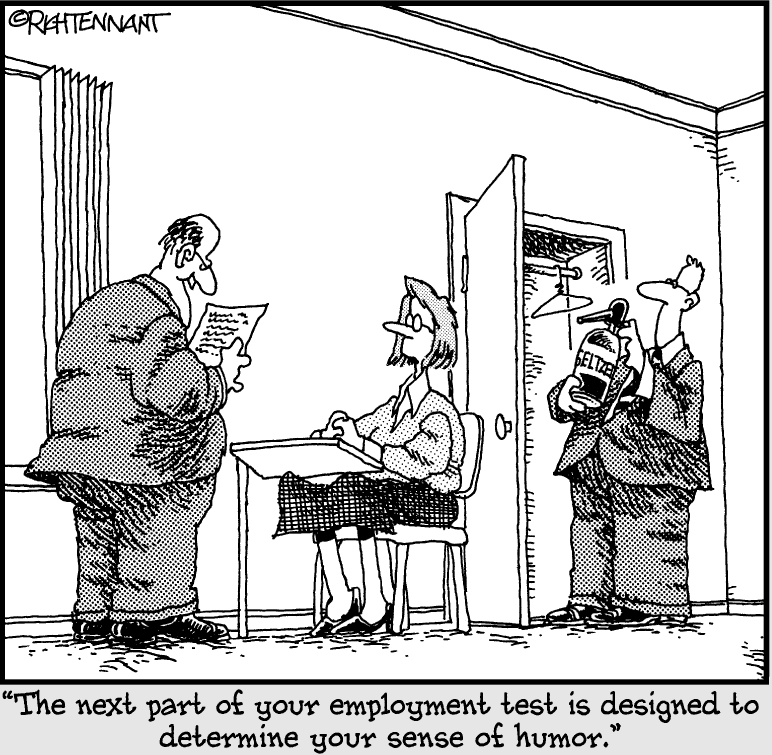
\includegraphics[scale=1.5]{figures/balancedscorecard_sensofhumor} \\
	%	\caption{Strategic management process}
	\label{balancedscorecard_sensofhumor} 
\end{figure}
\subsection{Background}


%\begin{shadequote}
\epigraph{"People in the engineering consultancy have to be tough and really resilient, if they are to survive in the climate which we work in"}%{--- \textup{}}
%\end{shadequote}

\paragraph{Some questions are to be considered}
\begin{itemize}
\item Where is engineering consultancy now and what changes have happened in the market during recent years?
\item What is happening in the wider world of all service industries and employment; what innovations are being tried out and how do these work in practice?
\item How are future markets for Consulting Engineers changing?
\item How can Consulting Engineers adapt their working practices for the new market, for their performance objectives, and to meet the aspirations of their employees, clients and other stakeholders?
\end{itemize}

\paragraph{Main responses from market changes}
\begin{itemize}

\item Clients have started to make it clear that they prefer to deal with the "expert" rather than the manager of any section of the business. As a result, firms have had to employ more experts in a front line role and increase their range of in-house disciplines;

\item Geographical demand and network requires local availability of experts;

\item Computerization and the Internet of things make it possible to perform rapid online design works and as well outsourcing;

\item Fees have fallen in response to market and competitive pressures. This has tended to reduce the input that firms have been willing to invest in a project, perhaps also limiting their ability to be creative;

\item Companies have become more professional in their marketing approaches and have had to engage in a much wider dialogue with clients as to their real business needs. Only can they put the appropriate expert in front of the client who will, hopefully, finalize the brief and, hence, the commission.

\end{itemize}


\epigraph{"the market pressures have led to an increased willingness by Consulting Engineering firms to collaborate with one another so as to optimize their skills and share costs in the face of a demanding client base"}%{--- \textup{}}

The dispersion of multi-disciplines offices poses a significant challenges in organizing the activities of the company in term of
\begin{itemize}
\item project performance, including scheduling, quality, costs, resources;
\item financial performance and cash management;
\item marketing, business promotion and development;
\item future planning strategies.
\end{itemize}

All of these need to reflect both the locational aspects of the different offices as well as their particular skills and resource availability.

\paragraph{Common themes}
\begin{itemize}
\item the importance of communicating with, and relating to, clients and the general public;
\item the need to value staff and their skills and thus achieve effective staff participation in the business;
\item new ways of assessing company performance overall and ensuring long-term viability;
\item building new relationships and alliances everywhere;
\item working in new ways to suit the IT and Internet of things age;
\item embarking on new ways of being involved in projects;
\item ongoing training for all;
\item broadening the skill and client bases through the acquisition of, or merger with, competitors;
\item partnering and alliances are seen very often as the way forward for many companies trying to be involved in large projects;
\item there is an increasing tendency for companies to have to take a financial stake in large projects;
\item profitability levels, almost everwhere, and certain amongst international competitor consultants, are generally modest.

\end{itemize}

\epigraph{"The factory of the future will have only two employees, a man and a dog. The man will be there to feed the dog. The dog will be there to keep the man from touching the equipment." }{---Warren Bennis}

This quotes implies that the system drives people, not the other way around. The factory and its process equipment has to be planned, designed, managed and constructed in the first place, and there will be always be an ongoing facilities management and maintenance requirement which consultants might take charge of.

\subsection{Organizational and management structures}
\begin{itemize}
\item Downsizing, the core worker concept: "half as many staff working twice as hard and producing three times as much!";
\item Flat management structures and restructuring: Toward TQM management goal, where "everyone is both a customer and a contractor, internally and externally". The trend will almost certainly continue as workers on increased responsibility for the commercial as well as technical aspects of businesses; clients are increasingly demanding a balanced approach between the technical and the cost (commercial) side of any service, so that the single focus point of contact must have full responsibility for both aspects;
\item localization and regionalisation;
\item partnering and alliances
\end{itemize}

\subsection{Working methods}
\begin{itemize}
\item Shamrock organization which has three level of leaves: (1) a central core of highly paid individuals; (2) a contracted fringe who works on project based scheme; and (3) hired outsiders during peak workload;
\item Portfolio working and the third age;
\item teleworking: \textit{"Joe has gone home to finish that report in peace and quiet, without interruptions - he'll be in on Friday when it's finished"};
\item the flexible office and the hot desk;
\end{itemize}

\subsection{Employment arrangements}
\begin{itemize}
\item Staff ownership and employee participation
\epigraph{the business reason "doing better can only be archived through our people. Our people must be given the freedom to apply their professional skills and business acumen in a way that keeps them a step ahead of our competitors", this means giving them a stake in the business}{}
\item The team approach: A shared leadership role infers (1) individual \& mutual accountability; (2) collective work products; (3) open discussions for all team members; all are active in problem solving; (4) common, agreed-on approach to completing work. All agree critical delivery points and costs.

\item employment contracts and incentivisation;

\item training and career development: employee needs to see where they want to go; where they see that the company is going; and are they content and confident with both?

\epigraph{Our resume with experience is like a bottle of milk, with expiry date. The expiry date for a milk bottle is about a week and the expiry date for us is about 3-4 years. Thus, if we do not update and learn, we will be soon out of the workforce}{Nam Le}
\end{itemize}

\subsection{Management of changes}
\epigraph{Companies cannot own people's intelligence; that belongs to the individuals concerned, and they need to be persuaded and encouraged to use it, in a continuing and more dedicated way, on behalf of the employing organization. Failure to provide appropriate employment framework will not provide that encouragement and they will go or drift elsewhere, taking not only their skills, but probably also their clients with them}{}

\epigraph{It is a combination of this new freedom of key employees, coupled with the Information Technology Revolution and the more open, demanding and competitive markets throughout the worl, that is the catalyst to continuous and significant change in all service industries}{}

\section{Market requirements}

\epigraph{For industrial and other private sector projects, it will increasingly be the project-management skills that will be the main driving force in the client's procurement strategy, rather than pure technical ability. Again, this will impact on the importance of this discipline in comparison with more technical skills within firms }{}

Consultants shall be well prepared for:

\begin{itemize}
\item new attitudes amongst technical and managerial staff;
\item new roles and forms of project involvement;
\item acceptance of different risks;
\item new relationships with other companies and with different forms of clients;
\item greater financial involvement in projects.
\end{itemize}

These types of trend will be the foundation for new strategies for Consulting Engineers.


\section{Strategies for Engineering Consultants}
\subsection{Strategy cycle}


\epigraph{The preparation of business strategies is always an ongoing process and an iterative one; it is not an activity that can be done once, then filed away}{}

\begin{figure}[!htb]
	%	\includepdf[angle = 0]{sections/CHE_1PHSC_with_VFD.pdf}
	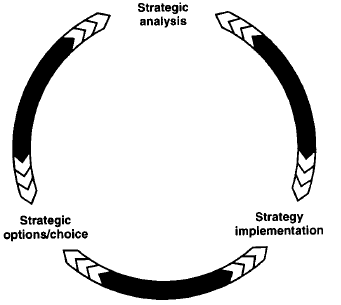
\includegraphics[scale=2]{figures/strategicmanagementprocess} \\
	\caption{Strategic management process}
	\label{strategicmanagementprocess} 
\end{figure}



\begin{figure}[!htb]
	%	\includepdf[angle = 0]{sections/CHE_1PHSC_with_VFD.pdf}
	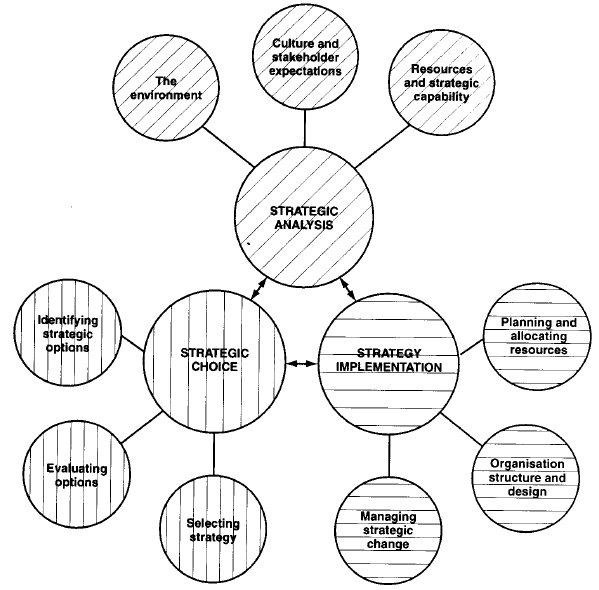
\includegraphics[scale=2]{figures/elementsinstrategicmanagement} \\
	\caption{Elements in strategic management}
	\label{elementsinstrategicmanagement} 
\end{figure}

\subsection{Scope of activities and the market climate}
\begin{itemize}
\item First step in the strategy: Evaluation/Assessment;
\item New services/new clients;
\item Selection of activities: (1) FS and advisory work; (2) Outline design; (3) Detailed engineering designs; (4) project management; (5) construction supervision; (6) facilities and operations management.
\end{itemize}

\subsection{The skill of the people}

\subsection{Company culture and attitudes}
\begin{itemize}
\item Corporate work culture;
\item Attitudes of staff;
\item Participation and rewards;
\item Working practices and stress;
\item Attitudes to changes;
\epigraph{All companies need to build this culture, yet it must sound risky to management and, to some extent, it is; and it will take time. But when people feel involved in a meaningful way, then they do not only easily go along with change, it is they who initiate it.}{}

\end{itemize}

\section{The organization of engineering consultancies in the future}

%\subsection{Management and organizational structures}

There are 3 factors in organizing a large and/or international business such as engineering consultancy
\begin{itemize}
\item an organizational structure which produces internal synergy;
\item a structure that encourage co-operative internal alliances, as well as external alliances with suppliers and customers, or even with competitors in the interest of keeping close to a particular client;
\item a structure that maintains a steady flow of new ideas about new products and new ventures for the company as a whole.
\end{itemize}










\end{document}
